\chapter{Results}
In this chapter we will present our overall results, by showing our training data, the hyper-parameters used, and
explain what worked and did not work.
Afterwards we will evaluate the best models and present our evaluation data.
\section{Training Experiments}
In \textbf{PPO} there are a number of hyper parameters that can be tweaked to achieve convergence.
An overview of the general parameters used can be seen in Table \ref{tab:hyper}.
\begin{table}[!ht]
    \begin{tabularx}{\linewidth}{lllX}
        \toprule
        Name & Value Used & Method & Description
        \\
        \midrule
        Hands Played & {[}5000,10000,15000{]} & Varied & The number of data points that go into each
        episode. Hands * 4 * 8 \\
        Batch Size & 80\% of the data & Fixed & The absolute size is dependent on the number of
        hands played \\
        Epochs & {[}8,12,16{]} & Varied & Number of Epochs(K) per episode
        \\
        Learning Rate & 0.0002 & Fixed & Used for Adams Optimiser
        \\
        Learning Rate Gamma & 0.3 & Fixed & Learning rate
        \\
        Clipping Range & 0.2 & Fixed & Clipping range to mange the clip the incremental
        change \\
        Discount Factor & 0.99 & Fixed & Used to calculate Discounted Rewards for
        Non-Terminal steps \\
        Value Function Coefficient & 0.5 & Fixed & (c1) Coefficent that allows computation of a
        comibined loss for actor-critic \\
        Entropy Coefficient        & 0.005            & Fixed  & (c2) Stops the model from early convergence
        \\
        Optimiser Weight Decay     & 1e-5             & Fixed  & Weight decay used in Adams Optimiser
        \\
        \bottomrule
    \end{tabularx}
    \caption{Hyperparameters used throughout the training.}
    \label{tab:hyper}
\end{table}

\subsection{CompleteRL}
For CompleteRL we experimented a fair bit with batch different values of the amount of hands played and it quickly
became apparent that CompleteRL was highly dependent on that number to be large.\\
Anything under 10000 (batch size = 256000,K=16) would simply not converge, and the distribution entropy was hovering
around 0.8, which means that the probabilities of actions effectively represented that of the Random agent.\\
Potential adjustment of the hyper-paramaters might solve this, but we doubt that.
\newline
One experiment that was successful was running 150000 hands(batch size=300000,K=16) over 80 steps.
Fig. \ref{fig:15comp} shows the achieved training progress.
\begin{figure}[!ht]
    \centering
    \subfloat[][Policy Loss]{\includegraphics[width=.4\textwidth]{15com/Loss_policy_loss}}\quad
    \subfloat[][Entropy]{\includegraphics[width=.4\textwidth]{15com/Loss_value_loss}}\\
    \subfloat[][Value Loss]{\includegraphics[width=.4\textwidth]{15com/Loss_entropy}}\quad
    \subfloat[][Explained Variance]{\includegraphics[width=.4\textwidth]{15com/Loss_avg_explained_var}}
    \caption{CompleteRL with 15000 hands per episode and K=16}
    \label{fig:15comp}
\end{figure}

\subsection{SeperatedRL}
For the training of \textbf{SepereratedRL} we experimented with smaller networks as our intuiton was that since we
train each gamemode individually less data might suffice.
CompleteRL for example only sees around 6\% Colo-Solos per episode, so the network a with 15000 hands might only sees
600 hands, that might get lost in the noise of all the other hands.
We therefore trained SeperatedRL with only 500 hands per episode (batch size =16000,K=8) and still managed to
reach convergence over 100 episodes.
\begin{figure}[!ht]
    \centering
    \subfloat[][Policy Loss]{\includegraphics[width=.4\textwidth]{500sad/Loss_policy_loss}}\quad
    \subfloat[][Entropy]{\includegraphics[width=.4\textwidth]{500sad/Loss_value_loss}}\\
    \subfloat[][Value Loss]{\includegraphics[width=.4\textwidth]{500sad/Loss_entropy}}\quad
    \subfloat[][Explained Variance]{\includegraphics[width=.4\textwidth]{500sad/Loss_avg_explained_var}}
    \caption{SeperateRL with 500 hands per episode and K=8.(blue=Team,red=Solo,grey=Wenz)}
    \label{fig:500sep}
\end{figure}


\section{Playing strength}
We now show the data of the latest episode in play against our baselines.
For each agent we played 10000 hands in a fair tournament that controls for the seeding, to ensure minimal variance.

\subsection{CompleteRL}
When we look at Table \ref{tab:evCompleteRL} we can see that CompleteRL was only able to beat the Random agent,
whilst losing against the other two by a good margin.
\newline


\begin{table}[]
    \centering
    \begin{tabular}{lccc}
        \toprule
        Player     & Random & Greedy & Heuristic \\
        \midrule
        CompleteRL & 2.11   & -1.63  & -2.65     \\
        \bottomrule
    \end{tabular}
    \caption{EV Overall: CompleteRL versus the baselines}
    \label{tab:evCompleteRL}
\end{table}

\begin{table}
    \begin{tabular}{lrrrrrrr}
        \toprule
        {}          & Team & Wenz & Solo & Team-Partner & Sauspiel-Opp & Wenz-Opp & Solo-Opp \\
        \midrule
        CompleteRL1 & 0.75 & 0.56 & 0.72 & 0.74         & 0.20         & 0.29     & 0.16     \\
        heu1        & 0.79 & 0.78 & 0.89 & 0.80         & 0.25         & 0.37     & 0.21     \\
        CompleteRL2 & 0.75 & 0.54 & 0.75 & 0.74         & 0.20         & 0.29     & 0.17     \\
        heu2        & 0.79 & 0.79 & 0.89 & 0.80         & 0.25         & 0.37     & 0.21     \\
        \bottomrule
    \end{tabular}
    \caption{Winrates: CompleteRL against Heuristic agent}
    \label{tab:table}
\end{table}

\begin{table}
    \begin{tabular}{lrrrrrrr}
        \toprule
        {}          & Team & Wenz & Solo & Team-Partner & Sauspiel-Opp & Wenz-Opp & Solo-Opp \\
        \midrule
        CompleteRL1 & 0.76 & 0.56 & 0.85 & 0.76         & 0.18         & 0.33     & 0.12     \\
        Greedy1     & 0.81 & 0.72 & 0.89 & 0.82         & 0.24         & 0.39     & 0.13     \\
        CompleteRL2 & 0.76 & 0.56 & 0.85 & 0.76         & 0.18         & 0.33     & 0.12     \\
        Greedy2     & 0.81 & 0.72 & 0.89 & 0.82         & 0.24         & 0.39     & 0.13     \\
        \bottomrule
    \end{tabular}
    \caption{Winrates: CompleteRL against Greedy agent}
    \label{tab:greedyRL}
\end{table}

\begin{table}
    \begin{tabular}{lrrrrrrr}
        \toprule
        {}          & Team & Wenz & Solo & Team-Partner & Sauspiel-Opp & Wenz-Opp & Solo-Opp \\
        \midrule
        CompleteRL1 & 0.81 & 0.75 & 0.92 & 0.78         & 0.24         & 0.37     & 0.11     \\
        Random1     & 0.73 & 0.55 & 0.85 & 0.79         & 0.20         & 0.30     & 0.09     \\
        CompleteRL2 & 0.81 & 0.77 & 0.95 & 0.77         & 0.23         & 0.37     & 0.13     \\
        Random2     & 0.77 & 0.59 & 0.86 & 0.78         & 0.21         & 0.31     & 0.10     \\
        \bottomrule
    \end{tabular}
    \caption{Winrates: CompleteRL against Random agent}
    \label{tab:ranRL}
\end{table}

\subsection{SeperatedRL}
\begin{table}[]
    \centering
    \begin{tabular}{lccc}
        \toprule
        Player     & Random & Greedy & Heuristic \\
        \midrule
        CompleteRL & 1.89   & -4.02  & -4.34     \\
        \bottomrule
    \end{tabular}
    \caption{EV Overall: CompleteRL versus the baselines}
    \label{tab:evSeperateRL}
\end{table}

